%# -*- coding: utf-8-unix -*-
% !TEX program = xelatex
% !TEX root = ../thesis.tex
% !TEX encoding = UTF-8 Unicode
%%==================================================
%% chapter02.tex for SJTU Master Thesis
%% based on CASthesis
%% modified by wei.jianwen@gmail.com
%% Encoding: UTF-8
%%==================================================

\chapter{基于多任务学习的NL2SQL生成}
\label{chap:cnl2sql}

\section{研究问题}

在第\ref{chap:enl2sql}章中,我们结合了深度学习与深度强化学习来解决NL2SQL的问题。
但是,目前的所有研究都只是将英文的自然语言问题转换为机器可执行的SQL查询语句,而没有涉及到其他语种的自然语言。
在本章中,我们主要的研究问题就是研究如何将中文的自然语言问题转换为SQL查询语句。
其中最具挑战的地方就是怎样将中文自然语言转换为英文自然语言的任务与英文自然语言生成SQL查询语句有机地结合起来。

基于多任务学习的NL2SQL生成的模型的总输入表示为$x$,其包含由单词$w_{i}$组成的自然语言问题$w$以及由列名$c_{j}$组成的数据库单张表的模式 $c$(其中,列名$c_{j}$可由单个或多个单词组成)。
模型的输出为一条可执行的SQL查询语句$y$以及其在数据库中执行的结果$r$。
我们通过给出NL2SQL任务中一个典型的例子(如图\ref{fig:nl2sqlexample}所示)来进一步说明。

\begin{figure}[!htp]
    \centering
    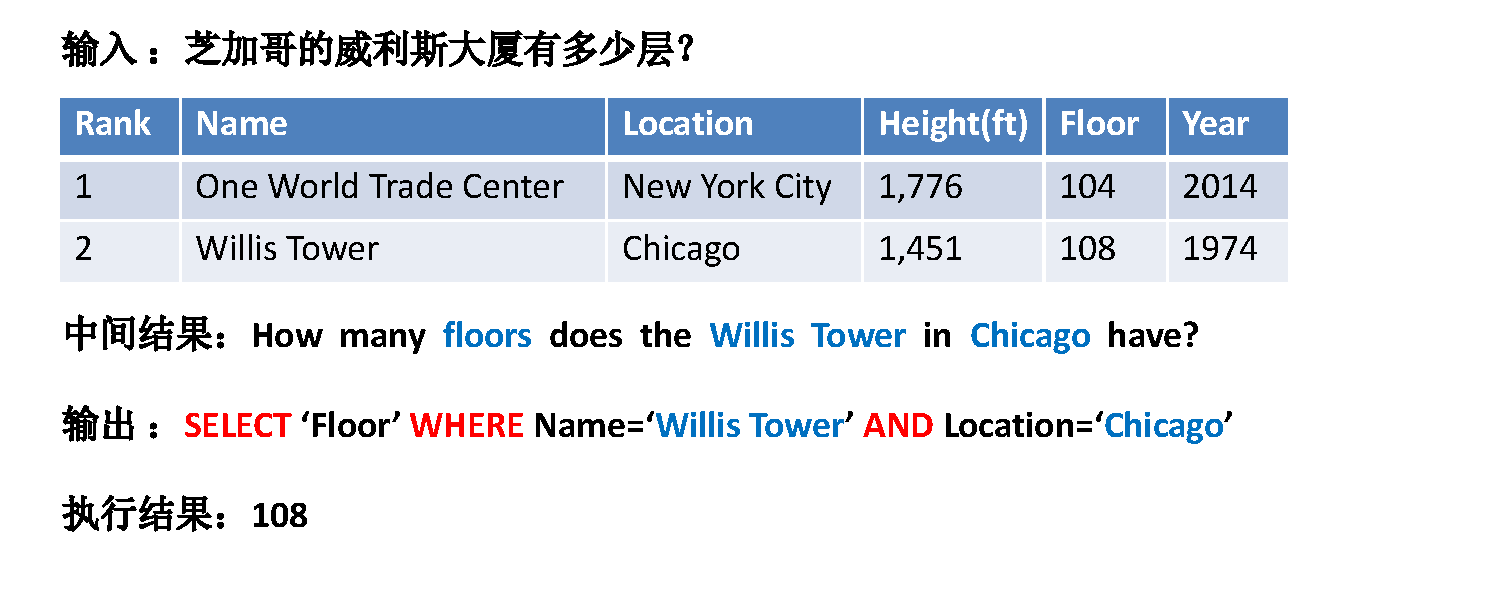
\includegraphics[width=17cm]{example/cnl2sql.pdf}
    \bicaption[这里将出现在插图索引中]
      {中文自然语言问题生成SQL查询语句的示例}
      {English caption}
    \label{fig:cnl2sqlexample}
  \end{figure}

在图\ref{fig:cnl2sqlexample}中,$w$代表中文自然语言问题“芝加哥的威利斯大厦有多少层?”,其中$w_0,w_1,w_2,...$分别代表单词“芝加哥”、“的”、“威利斯大厦”等。
$c$代表数据库表的模式“Name Location Height(ft) Floor Year”,其中$c_0,c_1,c_2,...$分别代表单词“Name”、“Location”、“Height(ft)”等。
总输入$x$代表由$w$和$c$组成的集合。
在将中文的自然语言问题转换为SQL查询语句的过程中会生成中间结果“How  many  floors  does  the  Willis  Tower  in  Chicago  have?”,即将中文翻译为英文,记作$m$。
模型的输出$y$在该示例中对应的SQL查询语句为“SELECT ‘Floor’ WHERE Name=‘Willis Tower’ AND Location=‘Chicago’”,其在数据库中执行的结果$r$为108。

基于多任务学习的NL2SQL生成的主要任务是要在将中文翻译为英文的同时,理解中文自然语言语句的意图并在一次交互的状态下将意图映射到SQL查询语句上,
即在知道数据库表模式$c$的状态下,将用户输入的自然语言问题$w$最终转换为一条SQL查询语句$y$并得到数据库执行结果$r$。

\section{相关技术}
\subsection{迁移学习与多任务学习}
\subsection{元学习}

\section{解决方案}

在本节中,我们会介绍如何把中文自然语言翻译为英文自然语言任务与英文自然语言生成SQL查询语句任务进行统一,之后提出一种基于多任务学习的神经网络结构并解释说明为何这样的网络结构可以有效地解决中文自然语言问题生成SQL查询语句问题。

\subsection{TCR模板}

首先,中文自然语言问题生成SQL查询语句可以被划分为两个子任务:中文自然语言翻译为英文自然语言任务和英文自然语言问题生成SQL查询语句任务。
在第\ref{chap:enl2sql}章中,本文提出的基于深度强化学习的解决方案已经可以有效的解决NL2SQL问题,并且在WikiSQL数据集和spider数据集上有优异的表现。
所以,我们会有一个非常自然的想法,就是直接使用翻译工具或翻译软件将中文的自然语言问题直接转换为英文自然语言问题,之后再使用\ref{enl2sql:zqjxqmx}节中提出的增强解析器模型将英文自然语言转换为SQL查询语句。
但是,这种方法会遇到许多问题,如图\ref{fig:cnl2sqlproblem}所示(其中中文自然语言均使用谷歌翻译自动翻译为英文自然语言):

\begin{figure}[!htp]
    \centering
    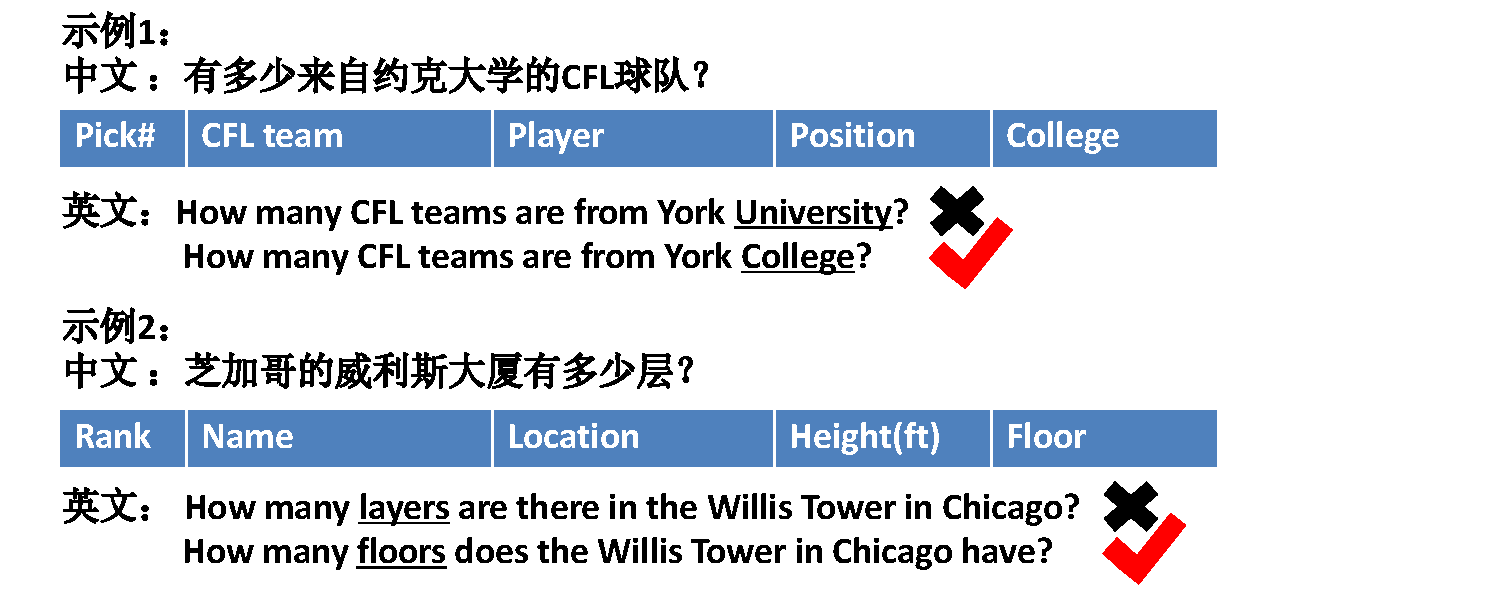
\includegraphics[width=17cm]{example/cnl2sqlproblem.pdf}
    \bicaption[这里将出现在插图索引中]
      {中文自然语言问题生成SQL查询语句的错误示例}
      {English caption}
    \label{fig:cnl2sqlproblem}
  \end{figure}

从图\ref{fig:cnl2sqlproblem}中的示例一可以看出,数据库表模式中的列名为“College”,而谷歌翻译将中文“大学”翻译为“University”。
而示例二中的“层”翻译为了“layers”而不是“floors”。
形如这一类的问题会给SQL的生成带来很大的问题。

究其原因,从中文自然语言到英文自然语言再到SQL查询语句这一过程是一个紧密关联的过程,如果将其拆分为两个部分,则翻译的过程中将会丢失大量的数据库、SQL语言本身的很多信息。
所以,我们提出TCR模板用以将这两个独立的任务有机的统一起来,并在作为下节中的多任务学习网络的输入。

\begin{figure}[!htp]
    \centering
    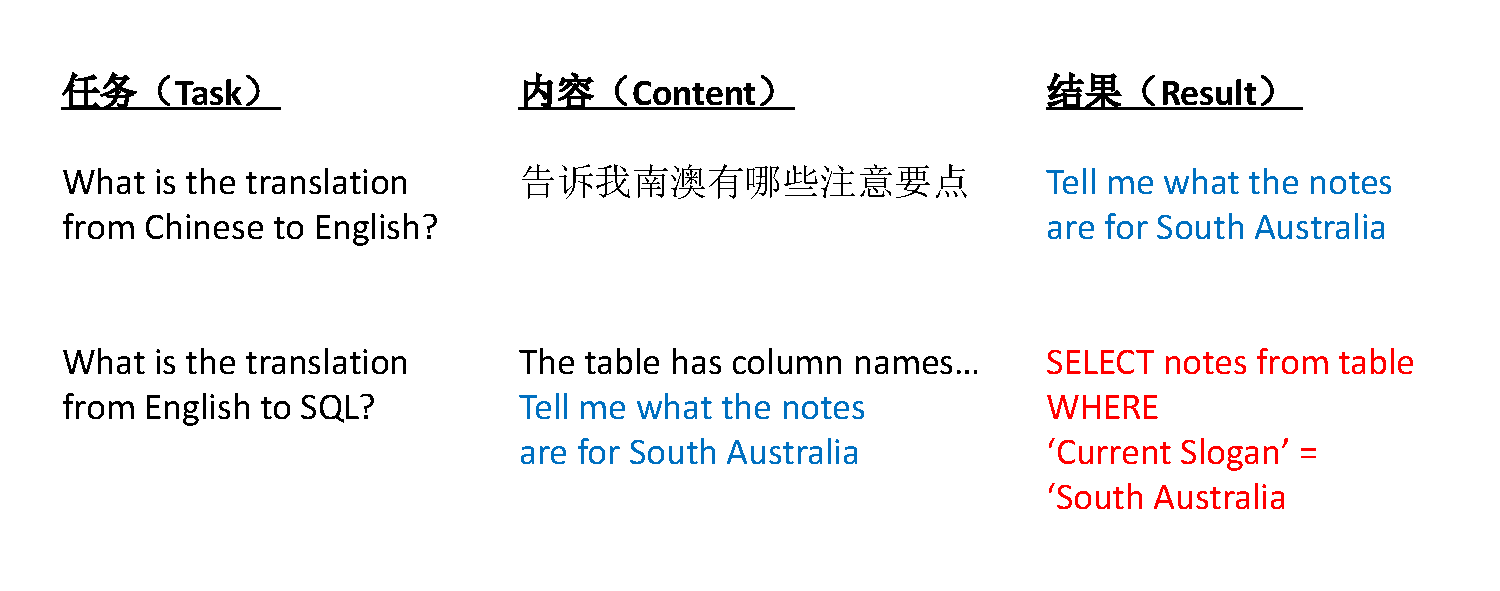
\includegraphics[width=17cm]{example/tcr.pdf}
    \bicaption[这里将出现在插图索引中]
      {TCR模板(任务-内容-结果模板)}
      {English caption}
    \label{fig:cnl2sqltcr}
  \end{figure}

如图\ref{fig:cnl2sqltcr}所示,我们将中文自然语言翻译为英文自然语言任务和英文自然语言生成SQL查询语句任务使用TCR模板(任务-内容-结果)进行统一。
例如,“告诉我南澳有哪些注意要点”先翻译为英文,其任务为“What is the translation from Chinese to English?”(意为需要执行的任务是中文到英文的翻译),内容为“告诉我南澳有哪些注意要点”(指在表明所需要翻译的中文自然语句是什么),结果为“Tell me what the notes are for South Australia”。
而后再将“Tell me what the notes are for South Australia”转换为SQL查询语句,其任务为“What is the translation from English to SQL?”(意为需要执行的任务是英文到SQL的生成),内容为“The table has column names… Tell me what the notes are for South Australia”(指在表明所需的信息由表的列名以及英文自然语言的查询构成),结果为“SELECT notes from table WHERE ‘Current Slogan’ =‘South Australia”,从而完成生成的全过程。

TCR模板将两个任务的模式进行了统一,使得网络模型的输入和输出得以一致,而不用设计两个不同的网络结构来处理这两个任务。
在后文中,我们还将这个模板用于自然语言处理领域中的很多任务,详见\ref{cnl2sql:syyfx}节。

\subsection{多任务网络}

由于我们会使用TCR模板对每个任务进行统一并且在训练阶段采用联合训练的方法,我们把所使用的神经网络的结构称为多任务网络,如图\ref{fig:cnl2sqlnet}所示。
近几年来,有许多研究者所研究的问答模型的和我们的模型比较类似,但是通常的问答模型往往假设模型得到的答案的片段是可以直接从上下文信息中复制,但是我们的多任务网络适用于更一般的问答场景。
在之前的TCR模板中,任务对应于问答模型中的问题,内容对应于问答模型中的上下文,而结果对应于问答模型中的回答。
由于TCR模板中的任务往往包含限制搜索空间的非常关键的信息,我们会在多任务网络中使用了协同注意力机制[!!引用!!]并加以拓展,从而使得对模型输入的表示更加丰富。
此外,多任务网络还采用了指针机制[!!引用!!],并将其改造为分层的多指针生成器,使得网络能够直接从任务和内容中进行文本的复制。

\begin{figure}[!htp]
  \centering
  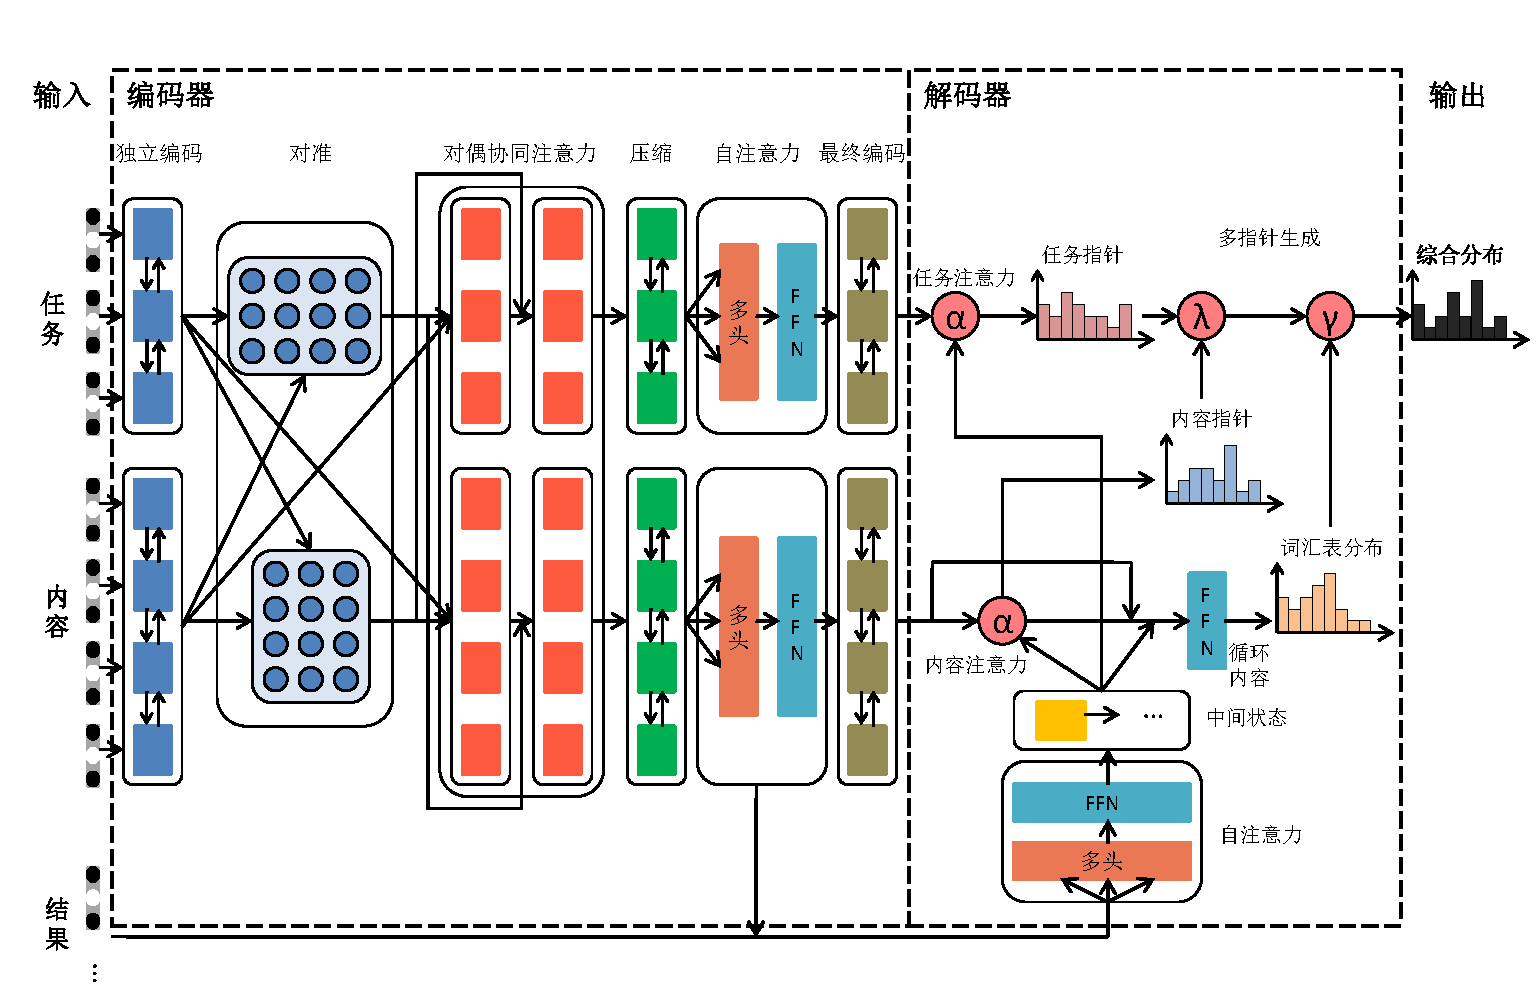
\includegraphics[width=17cm]{example/cnl2sqlnet.pdf}
  \bicaption[这里将出现在插图索引中]
    {多任务网络}
    {English caption}
  \label{fig:cnl2sqlnet}
\end{figure}

在训练阶段,多任务网络的输入序列会有三个部分,分别为:由$l$个单词构成的内容$c$;
由$m$个单词构成的任务$q$;由$n$个单词构成的结果$a$。
其中,每个输入序列都是一个矩阵,矩阵中的第$i$行对应于序列中的第$i$个词的嵌入(embedding)(可为字符向量或词向量),维度为$d_{emb}$。有公式\ref{cnl2sqleq:drwwl1}:
\begin{equation}
    \label{cnl2sqleq:drwwl1}
    C \in \mathbb{R}^{l \times d_{emb}} \qquad Q \in \mathbb{R}^{m \times d_{emb}} \qquad A \in \mathbb{R}^{n \times d_{emb}}
  \end{equation}

接下来,我们将分别详细介绍多任务网络中的编码器和解码器。

\subsection{编码器}
\label{cnl2sql:encoder}

编码器将内容矩阵$C$、任务矩阵$Q$和结果矩阵$A$作为输入,
使用深度栈式循环神经网络[!!引用!!],结合协同注意力机制(coattention)[!!引用!!]和自注意力机制(self-attention)[!!引用!!],
来生成编码阶段的最终的表示$C_{fin} \in \mathbb{R}^{l \times d}$和$Q_{fin} \in \mathbb{R}^{m \times d}$(即编码之后的内容信息和任务信息),
并且还可以让网络学习到他们之间的局部和全局的相互依赖关系。
在下文中,我们将对编码器的每个阶段进行进一步的说明。

\textbf{单独编码阶段}

首先使用一个简单的线性层将输入矩阵投射到$d$维的空间上,如公式\ref{cnl2sqleq:encoder1}。
\begin{equation}
    \label{cnl2sqleq:encoder1}
    CW_1 = C_{proj} \in \mathbb{R}^{l \times d} \qquad QW_1 = Q_{proj} \in \mathbb{R}^{m \times d} 
  \end{equation}
这些投射之后的表示将被输入给一个共享的双向长短期记忆网络(bi-LSTM)[!!引用!!][注释],如公式\ref{cnl2sqleq:encoder2}。
\begin{equation}
    \label{cnl2sqleq:encoder2}
    BILSTM_{ind}(C_{proj}) = C_{ind} \in \mathbb{R}^{l \times d} \qquad BILSTM_{ind}(Q_{proj}) = Q_{ind} \in \mathbb{R}^{l \times d}
\end{equation}

\textbf{对准阶段}

在获得协同注意力的表达之前,我们需要先对每个序列的编码表达进行对准。
我们会分别给$C_{ind}$和$Q_{ind}$增加一个预训练的嵌入使得现在的$C_{ind} \in \mathbb{R}^{(l+1) \times d}$以及$Q_{ind} \in \mathbb{R}^{(m+1) \times d}$,
这样做可以让每个单词不会和序列中的某个单词强制对准。

令$softmax(X)$表示逐列进行softmax操作,即矩阵$X$中的每列进行标准化后的和为1。
我们将内容信息的序列表示与任务序列表示之间进行点积计算得到相似性得分,并使用归一化操作来获得数据的对准,如公式\ref{cnl2sqleq:encoder3}:
\begin{equation}
  \label{cnl2sqleq:encoder3}
  softmax(C_{ind}Q_{ind}^{\top}) = S_{cq} \in \mathbb{R}^{(l+1) \times (m+1)} \qquad softmax(Q_{ind}C_{ind}^{\top}) = S_{qc} \in \mathbb{R}^{(m+1) \times (l+1)}
\end{equation}

\textbf{对偶协同注意力阶段}

再对准之后,我们要去计算一个序列中的某个单词和另一个序列中相关的单词的加权求和,如公式\ref{cnl2sqleq:encoder4}。
\begin{equation}
  \label{cnl2sqleq:encoder4}
  S_{cq}^{\top}C_{ind} = C_{sum} \in \mathbb{R}^{(m+1) \times d} \qquad S_{qc}^{\top}Q_{ind} = Q_{sum} \in \mathbb{R}^{(l+1) \times d}
\end{equation}

对偶协同注意力就是要通过同样的权重将对准时得到的信息传递给原序列,如公式\ref{cnl2sqleq:encoder5}。
\begin{equation}
  \label{cnl2sqleq:encoder5}
  S_{qc}^{\top}C_{sum} = C_{coa} \in \mathbb{R}^{(l+1) \times d} \qquad S_{cq}^{\top}Q_{sum} = Q_{coa} \in \mathbb{R}^{(m+1) \times d}
\end{equation}

可以发现,进行了加权求和和协同注意力的表示中的第一列为之前我们添加进去的冗余的嵌入。
在这里我们不再需要这一个嵌入,所以将矩阵中的这一列去除掉,得到$C_{coa} \in \mathbb{R}^{l \times d}$和$Q_{coa} \in \mathbb{R}^{m \times d}$。

\textbf{压缩阶段}

为了将对偶协同注意力操作之前的信息压缩至$d$维,我们接着把之前得到的四种序列表示进行拼接并输入一个单独的双向LSTM中,如公式\ref{cnl2sqleq:encoder6}。
\begin{align}
  \label{cnl2sqleq:encoder6}
  BiLSTM_{comC}([C_{proj};C_{ind};Q_{sum};C_{coa}]) =  C_{com} \in \mathbb{R}^{m \times d}\\
  BiLSTM_{comQ}([Q_{proj};Q_{ind};C_{sum};Q_{coa}]) =  Q_{com} \in \mathbb{R}^{m \times d}
\end{align}

\textbf{自注意力阶段}

接着,我们使用一个多头的放缩点积注意力机制(multi-head, scaled dot-product attention)[!!引用!!]来捕获每个序列内部的长距离的依赖性,其表达式为公式\ref{cnl2sqleq:encoder7}。

\begin{gather}
  \label{cnl2sqleq:encoder7}
  Attention(\widetilde{X},\widetilde{Y},\widetilde{Z}) = softmax\{\frac{\widetilde{X}\widetilde{Y}^{\top}}{\sqrt{d}}\} \widetilde{Z}\\
  MultiHead(\widetilde{X},\widetilde{Y},\widetilde{Z}) = [h_1;\cdots;h_p]W^o \qquad \mbox{其中}h_j= Attention(\widetilde{X}W^{\widetilde{X}}_j,\widetilde{Y}W^{\widetilde{Y}}_j,\widetilde{Z}W^{\widetilde{Z}}_j)
\end{gather}

公式\ref{cnl2sqleq:encoder7}中变换都为线性变换,所以多头注意力机制可以维持$d$维不变,有公式\ref{cnl2sqleq:encoder8}:
\begin{equation}
  \label{cnl2sqleq:encoder8}
  MultiHead_C(C_{com},C_{com},C_{com}) = C_{mha} \qquad MultiHead_Q(Q_{com},Q_{com},Q_{com}) = Q_{mha}
 \end{equation}

之后,我们使用了一个残差前馈网络(feedforward networks,简称FFN)如公式\ref{cnl2sqleq:encoder9},其中$U \in \mathbb{R}^{d \times f}$,$V \in \mathbb{R}^{f \times d}$。其激活函数为Relu函数[!!引用!!],并且在输入和输出都使用了正则化(layer normalization)[!!引用!!]。
\begin{gather}
  \label{cnl2sqleq:encoder9}
  FFN(X) = \max(0,XU)V + X\\
  FFN_C(C_{com} + C_{mha}) = C_{self} \in \mathbb{R}^{l \times d} \qquad FFN_Q(Q_{com} + Q_{mha}) = Q_{self} \in \mathbb{R}^{m \times d}
\end{gather}

\textbf{编码结束阶段}

最后,我们使用两个双向LSTM将所有信息进行汇总并将矩阵$C_{fin}$和$Q_{fin}$输入给解码器,如公式\ref{cnl2sqleq:encoder10}。
\begin{equation}
  \label{cnl2sqleq:encoder10}
  BiLSTM_{finC}(C_{self}) = C_{fin} \in \mathbb{R}^{l \times d} \qquad BiLSTM_{finQ}(Q_{self}) = Q_{fin} \in \mathbb{R}^{m \times d} 
\end{equation}


\subsection{解码器}
\label{cnl2sql:decoder}

在编码器得到最终的表示$C_{fin} \in \mathbb{R}^{l \times d}$和$Q_{fin} \in \mathbb{R}^{m \times d}$(即编码之后的内容信息和任务信息)后进入到解码器解码。
在下文中,我们将对解码器的每个阶段进行进一步的说明。

\textbf{结果表示阶段}

在训练阶段,解码器首先要将结果$a$的表示投射到$d$维的空间上,如公式\ref{cnl2sqleq:decoder1}

\begin{equation}
  \label{cnl2sqleq:decoder1}
  AW_2 = A_{proj} \in \mathbb{R}^{n \times d} 
\end{equation}

之后紧接的是一个自注意力层,该注意力层与编码器中的自注意力层相对应。
由于该过程不包含循环和卷积操作,所以我们为$A_{proj}$加上了一个位置编码信息$x$,如公式\ref{cnl2sqleq:decoder2}。
\begin{equation}
  \label{cnl2sqleq:decoder2}
  A_{proj} + PE = A_{ppr} \in \mathbb{R}^{n \times d},\qquad \mbox{其中} PE[t,k] = \{   
  \begin{array}{lr}
    sin(\frac{t}{10000^{\frac{k}{2d}}}) &  k\mbox{为偶数}\\
    cos(\frac{t}{10000^{\frac{k-1}{2d}}}) &  k\mbox{为奇数}
  \end{array}
\end{equation}

\textbf{自注意力阶段}
接着我们使用了自注意力机制[!!引用!!]从而使得解码器能够知道之前的输出(若之前没有输出则认为之前的输出为某个初始化的单词)和相关内容是什么,从而产生下一个输出。
在多头的注意力机制之后使用了一个残差前馈网络(FFN,其定义在\ref{cnl2sql:encoder}节中的自注意力阶段给出),如公式\ref{cnl2sqleq:decoder3}。

\begin{gather}
  \label{cnl2sqleq:decoder3}
  MultiHead_A(A_{ppr},A_{ppr},A_{ppr}) = A_{mha} \in \mathbb{R}^{n \times d}\\
  MultiHead_{A}C((A_{mha} + A_{ppr}),C_{fin},C_{fin}) = A_{ac} \in \mathbb{R}^{n \times d}\\
  FFN_A(A_{ac} + A_{mha} + A_{ppr}) = A_{self} \in \mathbb{R}^{n \times d}
\end{gather}

\textbf{获得中间状态阶段}

之后,我们使用了一个标准的带注意力机制的LSTM网络来对每个时刻$t$产生一个内容状态$\widetilde{c}_t$。
这个LSTM又将使用之前的结果序列中的单词$A^{t-1}_{self}$和内容状态来生成一个中间状态$h_t$,如公式\ref{cnl2sqleq:decoder4}。

\begin{equation}
  \label{cnl2sqleq:decoder4}
  LSTM([(A_{self})_{t-1};\widetilde{c}_{t-1}],h_{t-1})= h_t \in \mathbb{R}^{d} 
\end{equation}

\textbf{任务与内容注意力阶段}

上一阶段中的中间状态可用来获得注意力权重$\alpha^C_t$以及$\alpha^Q_t$Q,解码器从而可以获得$t$时刻的编码信息,如公式\ref{cnl2sqleq:decoder5}。

\begin{equation}
  \label{cnl2sqleq:decoder5}
  softmax(C_{fin}(W_2 h_t)) = \alpha^C_t \in \mathbb{R}^{l} \qquad softmax(Q_{fin}(W_3 h_t)) = \alpha^Q_t \in \mathbb{R}^{m}
\end{equation}

\textbf{获得内容与任务状态阶段}

内容的表示将于这些权重相结合并输入给一个前馈网络从而形成内容状态与任务状态,激活函数为$tanh$,如公式\ref{cnl2sqleq:decoder6}。
\begin{equation}
  \label{cnl2sqleq:decoder6}
  tanh(W_4[C^{\top}_{fin}\alpha^C_t;h_t] = \widetilde{c}_{t} \in \mathbb{R}^{d} \qquad tanh(W_5[Q^{\top}_{fin}\alpha^Q_t;h_t] = \widetilde{q}_{t} \in \mathbb{R}^{d}
\end{equation}

\textbf{多指针生成阶段}

由于我们的模型必须要能够生成那些未出现在任务或内容序列中的单词,所以需要额外声明一个词汇表$v$。
我们会从任务、内容和外部的词汇表中分别获得每个单词的概率分布,如公式\ref{cnl2sqleq:decoder7}。

\begin{gather}
  \label{cnl2sqleq:decoder7}
  \sum_{i:c_i=w_t} (\alpha^C_t)_i = p_c(w_t) \in \mathbb{R}^{n}\\
  \sum_{i:q_i=w_t} (\alpha^Q_t)_i = p_q(w_t) \in \mathbb{R}^{m}\\
  softmax(W_v\widetilde{c}_t) = p_v(w_t) \in \mathbb{R}^{v}
\end{gather}

这些概率分布将会覆盖任务、内容和外部词汇表中所有单词的集合,其中却是的一些条目将会被赋为0值从而使所有分布都在$\mathbb{R}^{l+m+v}$。
最后,我们设置两个标量开关来调节每个分布的重要程度并确认最终输出的分布,如公式\ref{cnl2sqleq:decoder8}。
\begin{gather}
  \label{cnl2sqleq:decoder8}
  \sigma (W_{pv}[\widetilde{c}_t;h_t;(A_{self})_{t-1}]) = \gamma \in [0,1]\\
  \sigma (W_{cq}[\widetilde{q}_t;h_t;(A_{self})_{t-1}]) = \lambda \in [0,1]\\
  \gamma p_v(w_t) + (1 - \gamma)[\lambda p_c(w_t) + (1 - \lambda)p_q(w_t)] = p(w_t) \in \mathbb{R}^{l+m+v}
\end{gather}

需要说明的是,在训练的全时域中,我们采用的是单词级别的对数似然损失,如公式\ref{cnl2sqleq:decoder9}。

\begin{equation}
  \label{cnl2sqleq:decoder9}
  \mathcal L = -\sum^T_t \log p(a_t)
\end{equation}























\section{实验与分析}
\label{cnl2sql:syyfx}
\section{本章小结}
Machine  ComprehensionQuestion answering (QA) mod-els receive a question and a context that contains informationnecessary  to  output  the  desired  answer.  We  use  the  StanfordQuestion  Answering  Dataset  (SQuAD)  []  for  this  task.  Con-texts  are  paragraphs  taken  from  the  English  Wikipedia,  andanswers  are  sequences  of  words  copied  from  the  context.SQuAD  uses  a  normalized  F1  (nF1)  metric  that  strip  outarticles and punctuation.Machine Translation.Machine translation models receivean  input  document  in  a  source  language  that  must  be  trans-lated  into  a  target  language.  We  use  the  2016  English  to

German training data prepared for the International Workshopon  Spoken  Language  Translation  (IWSLT)  [].  Examples  arefrom transcribed TED presentations that cover a wide varietyof  topics  with  conversational  language.  We  evaluate  with  acorpus-level BLEU score [] on the 2013 and 2014 test sets asvalidation and test sets, respectively.Natural  Language  Inference.Natural  Language  Infer-ence  (NLI)  models  receive  two  input  sentences:  a  premiseand  a  hypothesis.  Models  must  then  classify  the  inferencerelationship between the two as one of entailment, neutrality,or  contradiction.  We  use  the  Multi-Genre  Natural  LanguageInference Corpus (MNLI) [] which provides training examplesfrom  multiple  domains  (transcribed  speech,  popular  fiction,government  reports)  and  test  pairs  from  seen  and  unseen

domains.  MNLI  uses  an  exact  match  (EM)  score.  SentimentAnalysis.  Sentiment  analysis  models  are  trained  to  classifythe  sentiment  expressed  by  input  text.  The  Stanford  Senti-ment  Treebank  (SST)  []  consists  of  movie  reviews  with  thecorresponding  sentiment  (positive,  neutral,  negative).  We  usethe unparsed, binary version []. SST also uses an EM score.Semantic  Parsing.SQL  query  generation  is  related  tosemantic  parsing.  Models  based  on  the  WikiSQL  dataset[]  translate  natural  language  questions  into  structured  SQLqueries  so  that  users  can  interact  with  a  database  in  naturallanguage. WikiSQL is evaluated by a logical form exact match(lfEM)  to  ensure  that  models  do  not  obtain  correct  answersfrom incorrectly generated queries.Summarization.Summarization models take in a documentand  output  a  summary  of  that  document.  Most  important  torecent  progress  in  summarization  was  the  transformation  ofthe CNN/DailyMail (CNN/DM) corpus [Hermann et al., 2015]into  a  summarization  dataset  [Nallapati  et  al.,  2016].  We  in-clude the non-anonymized version of this dataset in decaNLP.On  average,  these  examples  contain  the  longest  documentsin decaNLP and force models to balance extracting from thecontext  with  generation  of  novel,  abstractive  sequences  ofwords.  CNN/DM  uses  ROUGE-1,  ROUGE-2,  and  ROUGE-L  scores  [Lin,  2004].  We  average  these  three  measures  tocompute an overall ROUGE score.Sentiment Analysis.Sentiment analysis models are trainedto classify the sentiment expressed by input text. The StanfordSentiment  Treebank  (SST)  [Socher  et  al.,  2013]  consists  ofmovie  reviews  with  the  corresponding  sentiment  (positive,neutral, negative). We use the unparsed, binary version [Rad-ford et al., 2017]. SST also uses an EM score.Semantic  Role  Labeling.Semantic  role  labeling  (SRL)models  are  given  a  sentence  and  predicate  (typically  a  verb)and must determine who did what to whom, when, and where[Johansson  and  Nugues,  2008].  We  use  an  SRL  dataset  thattreats  the  task  as  question  answering,  QA-SRL  [He  et  al.,2015]. This dataset covers both news and Wikipedia domains,but  we  only  use  the  latter  in  order  to  ensure  that  all  datafor decaNLP can be freely downloaded. We evaluate QA-SRLwith the nF1 metric used for SQuAD.Relation Extraction.Relation extraction systems take in apiece  of  unstructured  text  and  the  kind  of  relation  that  is  tobe extracted from that text. In this setting, it is important thatmodels can report that the relation is not present and cannot beextracted. As with SRL, we use a dataset that maps relations toa set of questions so that relation extraction can be treated asquestion answering: QA-ZRE [Levy et al., 2017]. Evaluationof  the  dataset  is  designed  to  measure  zero  shot  performanceon new kinds of relations   the dataset is split so that relationsseen  at  test  time  are  unseen  at  train  time.  This  kind  of  zero-shot relation extraction, framed as question answering, makesit  possible  to  generalize  to  new  relations.  QA-ZRE  uses  acorpus-level  F1  metric  (cF1)  in  order  to  accurately  accountfor unanswerable  questions. This F1  metric  defines precisionas  the  true  positive  count  divided  by  the  number  of  timesthe  system  returned  a  non-null  answer  and  recall  as  the  true

positive  count  divided  by  the  number  of  instances  that  havean answer.Goal-Oriented   Dialogue.Goal-Oriented  Dialogue.  Dia-logue  state  tracking  is  a  key  component  of  goal-orienteddialogue  systems.  Based  on  user  utterances,  actions  takenalready, and conversation history, dialogue state trackers keeptrack of which predefined goals the user has for the dialoguesystem  and  which  kinds  of  requests  the  user  makes  as  thesystem  and  user  interact  turn-by-turn.  We  use  the  EnglishWizard of Oz (WOZ) restaurant reservation task [Wen et al.,2016],  which  comes  with  a  predefined  ontology  of  foods,dates, times, addresses, and other information that would helpan agent make a reservation for a customer. WOZ is evaluatedby turn-based dialogue state EM (dsEM) over the goals of thecustomers.Semantic   Parsing.SQL  query  generation  is  related  tosemantic  parsing.  Models  based  on  the  WikiSQL  dataset[Zhong et al., 2017] translate natural language questions intostructured  SQL  queries  so  that  users  can  interact  with  adatabase  in  natural  language.  WikiSQL  is  evaluated  by  alogical  form  exact  match  (lfEM)  to  ensure  that  models  donot obtain correct answers from incorrectly generated queries.Pronoun  Resolution.Our final task is based on Winogradschemas  [Winograd,  1972],  which  require  pronoun  resolu-tion:  ”Joan  made  sure  to  thank  Susan  for  the  help  she  had[given/received].  Who  had  [given/received]  help?  Susan  orJoan?”.  We  started  with  examples  taken  from  the  WinogradSchema Challenge [Levesque et al., 2011] and modified themto  ensure  that  answers  were  a  single  word  from  the  context.This modified Winograd Schema Challenge (MWSC) ensuresthat  scores  are  neither  inflated  nor  deflated  by  oddities  inphrasing  or  inconsistencies  between  context,  question,  andanswer. We evaluate with an EM score.The  Decathlon  Score  (decaScore).Models  competing  ondecaNLP are evaluated using an additive combination of eachtask-specific metric. All metrics fall between 0 and 100, so thatthe decaScore naturally falls between 0 and 1000 for ten tasks.Using  an  additive  combination  avoids  issues  that  arise  fromweighing different metrics. All metrics are case insensitive.As shown in Table II. All metrics are case insensitive. nF1is  the  normalized  F1  metric  used  by  SQuAD  that  strips  outarticles  and  punctuation.  EM  is  an  exact  match  comparison:for  text  classification,  this  amounts  to  accuracy;  for  WOZ  itis equivalent to turn-based dialogue state exact match (dsEM)and  for  WikiSQL  it  is  equivalent  to  exact  match  of  logicalforms (lfEM). F1 for QA-ZRE is a corpus level metric (cF1)that  takes  into  account  that  some  question  are  unanswerable.Precision is the true positive count divided by the number oftimes the system returned a non-null answer. Recall is the truepositive  count  divided  by  the  number  of  instances  that  havean answer.

Because  every  task  is  framed  as  question  answering  andtrained jointly, we call our model a multitask question answer-

ing  network  (MQAN).  Each  example  consists  of  a  context,question,  and  answer  as  shown  in  Fig.  1.  Many  recent  QAmodels  for  question  answering  typically  assume  the  answercan  be  copied  from  the  context  [Wang  and  Jiang,  2017,  Seoet  al.,  2017,  Xiong  et  al.,  2018],  but  this  assumption  doesnot  hold  for  general  question  answering.  The  question  oftencontains  key  information  that  constrains  the  answer  space.Noting this, we extend the coattention of [Xiong et al., 2017]to enrich the representation of not only the input but also thequestion.  Also,  the  pointer-mechanism  of  [See  et  al.,  2017]is generalized into a hierarchical, multi-pointer-generator thatenables  the  capacity  to  copy  directly  from  the  question  andthe context.During training, the MQAN takes as input three sequences:a  context  c  with  l  tokens,  a  question  q  with  m  tokens,  andan answer a with n tokens. Each of these is represented by amatrix where the ith row of the matrix corresponds to a demb-dimensional embedding (such as word or character vectors) forthe ith token in the sequence:

Encoder:
xxxxx
Decoder:
xxxxx